% ZHOU-SOURCE-PAGE: 95 PRINTED: 79

\begin{problem}{Amoeba population}
There is a one amoeba in a pond. After every minute the amoeba may die, stay the same,
split into two or split into three with equal probability. All its offspring, if it has any, will
behave the same (and independent of other amoebas). What is the probability the
amoeba population will die out?
\end{problem}

\begin{solution}
This is just another standard conditional probability problem once you realize
we need to derive the probability conditioned on what happens to the amoeba one
minute later. Let $P(E)$ be the probability that the amoeba population will die out and
apply the law of total probability conditioned on what happens to the amoeba one
minute later:

\[
\begin{aligned}
P(E)={}&P(E\vert F_1)P(F_1)+P(E\vert F_2)P(F_2)\\
&+\cdots+P(E\vert F_n)P(F_n).
\end{aligned}
\]

For the original amoeba, as stated in the question, there are four possible mutually
exclusive events each with probability $1/4$. Let's denote $F_1$ as the event the amoeba dies;
$F_2$ as the event that it stays the same; $F_3$ as the event that it splits into two; $F_4$ as the
event that it splits into three. For event $F_1$, $P(E\vert F_1)=1$ since no amoeba is left.
$P(E\vert F_2)=P(E)$ since the state is the same as the beginning. For $F_3$, there are two
amoebas; either behaves the same as the original one. The total amoeba population will
die only if both amoebas die out. Since they are independent, the probability that they
both will die out is $P(E)^2$. Similarly we have $P(E\vert F_4)=P(E)^3$. Plug in all the numbers,
the equation becomes $P(E)=1/4\cdot1+1/4\cdot P(E)+1/4\cdot P(E)^2+1/4\cdot P(E)^3$.
Solve this equation with the restriction $0<P(E)<1$, and we will get $P(E)=\sqrt{2}-1\approx0.414$
(The other two roots of the equation are $1$ and $-\sqrt{2}-1$).

\end{solution}

\begin{problem}{Candies in a jar}
You are taking out candies one by one from a jar that has 10 red candies, 20 blue candies,
and 30 green candies in it. What is the probability that there are at least 1 blue candy and
1 green candy left in the jar when you have taken out all the red candies?\footnote[16]{\emph{Hint:} If there are at least 1 blue candy and 1 green candy left, the last red candy must have been
removed before the last blue candy and the last green candy in the sequence of 60 candies. What is the
probability that the blue candy is the last one in the 60-candy sequence? Conditioned on that, what is the
probability that the last green candy is the last one in the 30-candy sequence (10 red, 20 green)? What if
the green candy is the last one in the 60-candy sequence?}
\end{problem}

\begin{solution}
At first look, this problem appears to be a combinatorial one. However, a conditional
probability approach gives a much more intuitive answer. Let $T_r$, $T_b$ and $T_g$

% ZHOU-SOURCE-PAGE: 96 PRINTED: 80
be the number that the last red, blue, and green candies are taken out respectively. To
have at least 1 blue candy and 1 green candy left when all the red candies are taken out,
we need to have $T_r<T_b$ and $T_r<T_g$. In other words, we want to derive
$P(T_r<T_b\cap T_r<T_g)$. There are two mutually exclusive events that satisfy $T_r<T_b$ and
$T_r<T_g$: $T_r<T_b<T_g$ and $T_r<T_g<T_b$.

\[
\therefore\quad P(T_r<T_b\cap T_r<T_g)=P(T_r<T_b<T_g)+P(T_r<T_g<T_b)
\]

$T_r<T_b<T_g$ means that the last candy is green ($T_g=60$). Since each of the 60 candies
are equally likely to be the last candy and among them 30 are green ones, we have
$P(T_g=60)=\dfrac{30}{60}$. Conditioned on $T_g=60$, we need $P(T_r<T_b\vert T_g=60)$. Among the 30
red and blue candies, each candy is again equally likely to be the last candy and there are
20 blue candies, so $P(T_r<T_b\vert T_g=60)=\dfrac{20}{30}$ and $P(T_r<T_b<T_g)=\dfrac{30}{60}\cdot\dfrac{20}{30}$. Similarly,
we have $P(T_r<T_g<T_b)=\dfrac{20}{60}\cdot\dfrac{30}{40}$.

Hence,

\[
\begin{aligned}
P(T_r<T_b\cap T_r<T_g)&=P(T_r<T_b<T_g)+P(T_r<T_g<T_b)\\
&=\frac{30}{60}\cdot\frac{20}{30}+\frac{20}{60}\cdot\frac{30}{40}=\frac{7}{12}.
\end{aligned}
\]

\end{solution}

\begin{problem}{Coin toss game}
Two players, $A$ and $B$, alternatively toss a fair coin ($A$ tosses the coin first, then $B$ tosses
the coin, then $A$, then $B\ldots$). The sequence of heads and tails is recorded. If there is a
head followed by a tail ($HT$ subsequence), the game ends and the person who tosses the
tail wins. What is the probability that $A$ wins the game?\footnote[17]{\emph{Hint:} condition on the result of $A$'s first toss and use symmetry.}
\end{problem}

\begin{solution}
Let $P(A)$ be the probability that $A$ wins; then the probability that $B$ wins is
$P(B)=1-P(A)$. Let's condition $P(A)$ on $A$'s first toss, which has $1/2$ probability of $H$
(heads) and $1/2$ probability of $T$ (tails).

\[
P(A)=1/2P(A\vert H)+1/2P(A\vert T)
\]

If $A$'s first toss is $T$, then $B$ essentially becomes the first to toss (An $H$ is required for the
$HT$ subsequence). So we have $P(A\vert T)=P(B)=1-P(A)$.

If $A$'s first toss ends in $H$, let's further condition on $B$'s first toss. $B$ has $1/2$ probability
of getting $T$, in that case $A$ loses. For the $1/2$ probability that $B$ gets $H$, $B$ essentially

% ZHOU-SOURCE-PAGE: 97 PRINTED: 81
becomes the first one to toss an $H$. In that case, $A$ has $(1-P(A\vert H))$ probability of
winning. So $P(A\vert H)=1/2\cdot0+1/2\cdot(1-P(A\vert H))\Rightarrow P(A\vert H)=1/3$

Combining all the available information, we have

\[
P(A)=1/2\cdot1/3+1/2(1-P(A))\Rightarrow P(A)=4/9.
\]

\emph{Sanity check:} we can see that $P(A)<1/2$, which is reasonable since $A$ cannot win in his
first toss, yet $B$ has $1/4$ probability to win in her first toss.

\end{solution}

\begin{problem}{Russian roulette series}
Let's play a traditional version of Russian roulette. A single bullet is put into a 6-chamber
revolver. The barrel is randomly spun so that each chamber is equally likely to be under the
hammer. Two players take turns to pull the trigger---with the gun unfortunately pointing at one's own head---without further spinning until the gun goes
off and the person who gets killed loses. If you, one of the players, can choose to go first
or second, how will you choose? And what is your probability of loss?
\end{problem}

\begin{solution}
Many people have the wrong impression that the first person has higher probability of loss.
After all, the first player has a $1/6$ chance of getting killed in the first round before the second
player starts. Unfortunately, this is one of the few times that intuition is wrong. Once the barrel is
spun, the position of the bullet is fixed. If you go first, you lose if and only if the bullet is in
chamber 1, 3 and 5. So the probability that you lose is the same as the second player, $1/2$. In that sense,
whether to go first or second does not matter.
\end{solution}

\begin{problem}{}
Now, let's change the rule slightly. We will spin the barrel again after every trigger pull.
Will you choose to be the first or the second player? And what is your probability of loss?
\end{problem}

\begin{solution}
The difference is that each run now becomes independent. Assume that the first player's
probability of losing is $p$, then the second player's probability of losing is $1-p$. Let's condition the
probability on the first person's first trigger pull. He has $1/6$ probability of losing in this run.
Otherwise, he essentially becomes the second player in the game with new (conditional) probability
of losing $1-p$. That happens with probability $5/6$. That gives us $p=1\cdot1/6+(1-p)\cdot5/6$
$\Rightarrow p=6/11$. So you should choose to be the second player and have $5/11$ probability of losing.
\end{solution}

\begin{problem}{}
If instead of one bullet, two bullets are randomly put in the chamber. Your opponent played the first and he was alive after the first trigger pull. You are given the option
whether to spin the barrel. Should you spin the barrel?
\end{problem}

% ZHOU-SOURCE-PAGE: 98 PRINTED: 82
\Needspace{4\baselineskip}
\begin{solution}
if you spin the barrel, the probability that you will lose in this round is $2/6$. If you don't spin the barrel, there are only 5 chambers left and your probability of losing in
this round (conditioned on that your opponent survived) is $2/5$. So you should spin the
barrel.
\end{solution}

\begin{problem}{}
What if the two bullets are randomly put in two consecutive positions? If your opponent
survived his first round, should you spin the barrel?
\end{problem}

\begin{solution}
Now we have to condition our probability on the fact that the positions of the two bullets are consecutive.
As shown in Figure 4.3, let's label the empty chambers as 1, 2, 3 and 4; label the ones with bullets
5 and 6. Since your opponent survived the first round, the possible position he encountered is 1, 2, 3 or 4
with equal probability. With $1/4$ chance, the next one is a bullet (the position is 4). So if you don't spin the barrel,
the chance of survival is $3/4$. If you spin the barrel, each position has equal probability of being
chosen, and your chance of survival is only $2/3$. So you should not spin the barrel.
\end{solution}

\begin{figure}[ht]
\centering
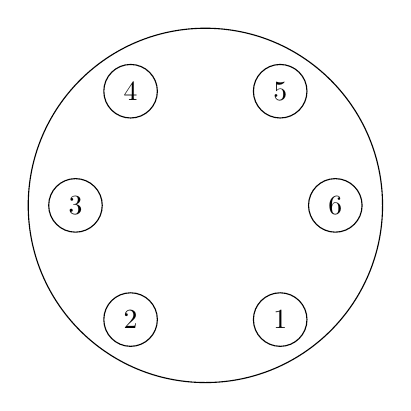
\begin{tikzpicture}[scale=1.0]
  \draw (0,0) circle (2.25cm);
  \foreach \x/\y/\n in {
    -0.95/1.45/4,
    0.95/1.45/5,
    -1.65/0/3,
    1.65/0/6,
    -0.95/-1.45/2,
    0.95/-1.45/1}
    {\draw (\x,\y) circle (0.34cm) node {\n};}
\end{tikzpicture}
\caption{Russian roulette with two consecutive bullets.}
\label{fig:zhou-figure-4-3}
\end{figure}

\begin{problem}{Aces}
Fifty-two cards are randomly distributed to 4 players with each player getting 13 cards.
What is the probability that each of them will have an ace?
\end{problem}

\begin{solution}
The problem can be answered using standard counting methods. To distribute
52 cards to 4 players with 13 cards each has $\dfrac{52!}{13!13!13!13!}$ permutations. If each player

% ZHOU-SOURCE-PAGE: 99 PRINTED: 83
needs to have one ace, we can distribute the aces first, which has $4!$ ways. Then we
distribute the rest 48 cards to 4 players with 12 cards each, which has
$\dfrac{48!}{12!12!12!12!}$ permutations. So the probability that each of them will have an Ace is

\[
4!\cdot\frac{48!}{12!12!12!12!}\div\frac{52!}{13!13!13!13!}
=\frac{52}{52}\cdot\frac{39}{51}\cdot\frac{26}{50}\cdot\frac{13}{49}.
\]

The logic becomes clearer if we use a conditional probability approach. Let's begin with
any one of the four aces; it has probability $52/52=1$ of belonging to a pile. The second
ace can be any of the remaining 51 cards, among which 39 belong to a pile different
from the first ace. So the probability that the second ace is not in the pile of the first ace
is $39/51$. Now there are 50 cards left, among which 26 belong to the other two piles. So
the conditional probability that the third ace is in one of the other 2 piles given the first
two aces are already in different piles is $26/50$. Similarly, the conditional probability
that the fourth ace is in the pile different from the first three aces given that the first
three aces are in different piles is $13/49$. So the probability that each pile has an ace is

\[
1\cdot\frac{39}{51}\cdot\frac{26}{50}\cdot\frac{13}{49}.
\]

\end{solution}

\begin{problem}{Gambler's ruin problem}
A gambler starts with an initial fortune of $i$ dollars. On each successive game, the
gambler wins \$1 with probability $p$, $0<p<1$, or loses \$1 with probability $q=1-p$.
He will stop if he either accumulates $N$ dollars or loses all his money. What is the
probability that he will end up with $N$ dollars?
\end{problem}

\begin{solution}
This is a classic textbook probability problem called the Gambler's Ruin Problem.
Interestingly, it is still widely used in quantitative interviews.

From any initial state $i$ (the dollars the gambler has), $0\leq i\leq N$, let $P_i$ be the probability
that the gambler's fortune will reach $N$ instead of 0. The next state is either $i+1$ with
probability $p$ or $i-1$ with probability $q$. So we have

\[
\begin{aligned}
P_i={}&pP_{i+1}+qP_{i-1}\Rightarrow P_{i+1}-P_i=\frac{q}{p}(P_i-P_{i-1})\\
&=\left(\frac{q}{p}\right)^2(P_{i-1}-P_{i-2})=\cdots\\
&=\left(\frac{q}{p}\right)^i(P_1-P_0)
\end{aligned}
\]

We also have the boundary probabilities $P_0=0$ and $P_N=1$.

So starting from $P_2$, we can successively evaluate $P_i$ as an expression of $P_1$:
\end{solution}
